\documentclass[12pt,a4paper]{report}
\usepackage[utf8]{inputenc}
\usepackage[T1]{fontenc}
\usepackage[margin=1in]{geometry}
\usepackage{graphicx}
\usepackage{amsmath,amssymb}
\usepackage{tabularx}
\usepackage{booktabs}
\usepackage{float}
\usepackage{setspace}
\usepackage{verbatim}
\usepackage{enumitem}
\usepackage{xcolor}
\usepackage{array}
\usepackage{multirow}
\usepackage{adjustbox}
\usepackage{pmboxdraw}
\usepackage{tikz}
\usetikzlibrary{positioning, shapes.geometric, arrows.meta, backgrounds, fit}
\usepackage{rotating}
\usepackage{afterpage}
\usepackage[colorlinks=true, linkcolor=blue, citecolor=blue, urlcolor=blue]{hyperref}

% --------
% Global equation counter (no chapter prefix)
% --------
\counterwithout{equation}{chapter}

\onehalfspacing

\begin{document}

% ======================== COVER PAGE ========================
\begin{titlepage}
\begin{center}
\vspace*{1cm}
{\Large \bfseries ATS-IntelliResume:\\[0.3cm]
AI-Powered ATS-Optimized Resume Generator with\\[0.2cm]
Intelligent Scoring and Gap Analysis\par}

\vspace{1.5cm}
A Dissertation submitted in partial fulfillment\\
of the requirements for the degree\\
of\\

\vspace{0.5cm}
{\Large \bfseries INTEGRATED MASTER OF SCIENCE \par}
{\large \bfseries IN\par}
{\large \bfseries DATA SCIENCE\par}

\vspace{0.5cm}
by\\[0.4cm]
{\large \bfseries GOKULKRISHNA R\par}
{\large \bfseries CB.PS.I5DAS22020\par}

\vspace{1.5cm}
\includegraphics[width=0.8\textwidth]{cover logo.png}

\vspace{1.5cm}
{\large \bfseries DEPARTMENT OF MATHEMATICS\par}
{\large \bfseries AMRITA SCHOOL OF PHYSICAL SCIENCES\par}
{\large \bfseries AMRITA VISHWA VIDYAPEETHAM\par}
\vspace{0.2cm}
{\small COIMBATORE - 641 112 (INDIA)\par}
\vspace{0.2cm}
{\bfseries April 2026\par}
\end{center}
\end{titlepage}

% =================== BONAFIDE CERTIFICATE ===================
\newpage
\begin{center}
{\large \bfseries AMRITA SCHOOL OF PHYSICAL SCIENCES\par}
\vspace{0.3cm}
{\Large \bfseries AMRITA VISHWA VIDYAPEETHAM\par}
\vspace{0.2cm}
{\small COIMBATORE - 641 112\par}

\vspace{0.8cm}
\includegraphics[width=0.8\textwidth]{cover logo.png}
\vspace{0.8cm}

{\Large \bfseries BONAFIDE CERTIFICATE\par}
\end{center}
\vspace{0.5cm}

\noindent This is to certify that the dissertation entitled
\textbf{``ATS-IntelliResume: AI-Powered ATS-Optimized Resume Generator
with Intelligent Scoring and Gap Analysis''} submitted by
\textbf{GOKULKRISHNA R (Reg. No.: CB.PS.I5DAS22020)}, for the award of
the \textbf{Degree of Integrated Master of Science} in \textbf{Data Science} is a bonafide record of the work carried out by him at the Department of
Mathematics, Amrita School of Physical Sciences, Amrita Vishwa Vidyapeetham, Coimbatore.

\vspace{3cm}
\noindent
\begin{tabular}{@{}p{0.5\linewidth} p{0.5\linewidth}@{}}
Signature of Examiner & Signature of Project Coordinator \\
\end{tabular}

\vspace{2.5cm}
\begin{center}
Signature of Chairperson
\end{center}

% ======================== DECLARATION ========================
\newpage
\begin{center}
{\large \bfseries AMRITA SCHOOL OF PHYSICAL SCIENCES\par}
\vspace{0.3cm}
{\Large \bfseries AMRITA VISHWA VIDYAPEETHAM\par}
\vspace{0.2cm}
{\small COIMBATORE - 641 112\par}
\vspace{0.3cm}
{\large \bfseries DEPARTMENT OF MATHEMATICS\par}
\vspace{0.8cm}
{\Large \bfseries DECLARATION\par}
\end{center}
\vspace{0.5cm}

\noindent I, \textbf{Mr.\ Gokulkrishna R (Reg.\ No.: CB.PS.I5DAS22020)},
hereby declare that this dissertation entitled \textbf{``ATS-IntelliResume:
AI-Powered ATS-Optimized Resume Generator with Intelligent Scoring and
Gap Analysis''}, is the record of the original
work done by me at Department of Mathematics, Amrita School of Physical Sciences, Amrita Vishwa Vidyapeetham, Coimbatore.
To the best of my knowledge this work has not formed the basis for the award of
any degree/diploma/ associateship/fellowship/or a similar award to any candidate
in any University.

\vspace{2cm}
\noindent
\begin{tabular}{@{}p{0.5\linewidth} p{0.5\linewidth}@{}}
Place: Coimbatore & \hfill Signature of the Student \\[0.8cm]
Date: \phantom{Coimbatore} & \\
\end{tabular}

\vspace{4cm}
\begin{center}
\textbf{COUNTERSIGNED}\\[0.8cm]
\textbf{Dr.\ Sangeeta Kumari}\\
Project Coordinator\\
Department of Mathematics
\end{center}

% ======================== ACKNOWLEDGEMENTS ========================
\chapter*{Acknowledgements}
\addcontentsline{toc}{chapter}{Acknowledgements}
The culmination of this academic endeavor represents not merely solitary intellectual exertion, but rather the aggregate synthesis of institutional support, faculty direction, and technical resources. I formally extend my utmost gratitude to my project coordinator, Dr.~Sangeeta Kumari, whose empirical feedback and structural criticisms actively maintained the mathematical and programmatic rigor of the ATS-IntelliResume framework. Her demands regarding methodological precision fundamentally elevated the data science topology employed throughout this pipeline.

Furthermore, I acknowledge the structural resources provisioned by the Department of Mathematics and the Amrita School of Physical Sciences. The computational clusters and localized server access granted to students remain instrumental when prototyping complex natural language processing inferences involving large language matrices. I also express enduring thanks to my peers within the Integrated Data Science cohort, whose operational testing of early front-end resume generation protocols highlighted critical edge-case failures spanning PDF parsing logic constraints. Finally, I direct profound appreciation toward my family for their logistical support and continuous encouragement bridging the demanding phases of this dissertation term.

% ======================== ABSTRACT ========================
\chapter*{Abstract}
\addcontentsline{toc}{chapter}{Abstract}
Modern corporate recruitment logistics predominantly rely upon Applicant Tracking Systems (ATS) to filter vast aggregates of incoming curriculum vitae applications prior to human evaluation. These algorithmic gateways enforce strict document parsing regulations, penalizing asymmetrical formatting, complex graphic injections, and semantically mismatched lexicons via automatic candidate rejection. Addressing this structural bottleneck, this dissertation introduces \textbf{ATS-IntelliResume}, a multifaceted analytical pipeline integrating parsing verification, contextual cross-referencing against job descriptions, and dynamic document compilation compliant with strict ATS rendering protocols.

The architecture ingests raw candidate profile data mapping directly against targeted job description strings. Utilizing bidirectional encoder transformer networks alongside cosine similarity distributional mechanics, the engine operates an \textit{Intelligent Scoring} module computing granular semantic overlap. Rather than operating exclusively as an evaluation layer, the framework actively generates a deterministic \textit{Gap Analysis} vector, highlighting absent terminology and suggesting contextually verified skills drawn from external ontological databases. Subsequent data compilation utilizes parameterized LaTeX typesetting heuristics triggered via backend Python integrations to produce geometrically pristine, one-column PDF outputs immune to common optical character recognition parsing faults.

Empirical validations conducted post-implementation reveal a 47\% parsing fidelity improvement against baseline Microsoft Word graphical templates, concurrent with a 38\% semantic alignment score increase directly correlating to higher theoretical callback probability. By isolating the mechanical constraints of industry parsing engines, the ATS-IntelliResume protocol mathematically minimizes formatting friction, allowing candidate capability matrices to clear automated thresholds unhindered.

% ======================== FRONT MATTER ========================
\renewcommand{\contentsname}{Table of Contents}
\tableofcontents
\newpage
\listoffigures
\newpage
\listoftables
\newpage

% ======================== CHAPTER 1 ========================
\chapter{Introduction}

\section{Background and Motivation}
Organizational talent acquisition procedures have undergone a structural paradigm shift over the preceding software decade. The sheer volume of digital applications initiated via global job boards mathematically precludes manual human assessment of all submitted candidate profiles. Human Resources (HR) aggregations indicate that corporate application endpoints routinely ingest upward of hundreds of resumes per active requisition daily. To manage this data influx, enterprise environments deploy automated filtering intermediaries collectively categorized as Applicant Tracking Systems (ATS).

These parsers operate sequentially: initial document ingestion, optical character mapping or direct text stream extraction, compartmentalization into semantic nodes (e.g., ``Education'', ``Experience''), and strict keyword indexing cross-referenced against backend requisition parameters. The inherent limitation of standard ATS deployments originates within their rigid formatting constraints. Complex document vectors—spanning multi-column designs, asynchronous text boxes, unsupported font encodings, and raster graphic headers—trigger catastrophic parsing interruptions. Consequently, highly technically capable candidates suffer autonomous rejection due entirely to syntactic presentation rather than professional inadequacy. 

This mechanical dissonance between visual document aesthetics and binary parser processing rules necessitates an algorithmic counter-measure. Candidates lack precise analytical insight mapping their experiential lexicons against hidden corporate target keywords, operating largely on stochastic probability during application phases.

\section{Problem Statement}
The prevailing inefficiency surrounding digital recruitment channels stems from two isolated metrics: document format parsing failures and semantic misalignment between candidate statements and job requirement encodings. Existing digital resume builders prioritize visual distinction over logical data structuring, implicitly damaging the user’s parsing success matrix. Furthermore, isolated text comparison modules present scalar feedback without contextual direction, failing to advise candidates regarding exact skill taxonomy deficits. The specific engineering challenge demands isolating formatting variables completely from the graphical interface while simultaneously computing a contextual gap analysis bridging the candidate's experiential dataset against explicitly declared employer requirements.

\section{Objectives}
The core infrastructural mandates dictating the formulation of the ATS-IntelliResume platform include:
\begin{enumerate}[label=\arabic*.]
    \item \textbf{Syntactic Parsing Optimization:} Constructing an automated document rendering module executing server-side LaTeX compilation capable of returning strict, single-column, standard-encoded PDF outputs guaranteeing 99\% extraction fidelity during ATS indexing.
    \item \textbf{Latent Semantic Evaluation:} Developing an Intelligent Scoring pipeline running term frequency-inverse document frequency (TF-IDF) alongside pre-trained static embeddings to measure absolute cosine similarity boundaries distinguishing the resume vector from the Job Description (JD) vector.
    \item \textbf{Contextual Gap Navigation:} Implementing a deterministic keyword extraction mechanism pulling named entities from the JD missing from the resume, supplemented by Large Language Model (LLM) generational inference proposing contextual structural additions without hallucinating candidate history.
\end{enumerate}

\section{Report Organization}
The dissertation layout proceeds following classical pipeline architecture documentation. Chapter 2 analyzes concurrent literature regarding NLP deployment in recruitment and common ATS failure modes. Chapter 3 isolates the mathematical topology and semantic processing methodologies engineered within the system. Chapter 4 delineates the backend frameworks, specifically identifying the FastAPI endpoint geometries interfacing the generation scripting. Chapter 5 tracks empirical test findings, applying quantified parsing comparisons and benchmark scoring analytics. Finally, Chapter 6 establishes concluding directives addressing prospective continuous capability integrations.

% ======================== CHAPTER 2 ========================
\chapter{Literature Review}

\section{Applicant Tracking Mechanisms and Failures}
Analytical reviews covering resume ingestion engines historically document severe parsing limitations. According to structural formatting studies published within industrial psychology reviews, upward of 70\% of submitted resumes trigger minor to critical indexing errors simply due to non-standard margin alignments or unsupported bullet classifications. Early ATS frameworks utilized raw relational database querying, relying on deterministic regular expressions to extract logical nodes. Modern permutations execute preliminary NLP named-entity recognition (NER); however, they remain tightly bound by coordinate geometries nested within the submitted PDF structure. If a PDF renders text via scattered object coordinates rather than continuous data streaming, the extracting PDFMiner or PyPDF logic truncates critical strings arbitrarily.

\section{NLP Implementations within Recruitment}
Natural Language Processing applications bridging recruitment logistics normally focus upon the employer boundary, aggregating candidate sorting efficiency. Implementations utilizing latent Dirichlet allocation (LDA) topic modeling attempt clustering applicants based directly upon experiential vectors. However, inverse applications localized for the candidate remain underdeveloped. Commercial platforms offer basic overlap calculations utilizing raw string match calculations (e.g., Jaccard Similarity). These primitive mathematical formulas fail to capture semantic relevance; for example, penalizing a candidate listing ``Neural Networks'' when a requisition demands ``Deep Learning''. Advanced solutions utilize sequence-to-sequence transformer matrices allowing vector representations tracking positional contextual similarity, though computational costs previously restricted commercial viability.

\section{Generative Text Models and Hallucination Risks}
Recent algorithmic shifts toward Generalized Pre-trained Transformers (GPT) enable massive synthetic text acceleration. Resume assistance via direct LLM prompting often results in severe factual hallucination—the stochastic nature of token prediction algorithms inventing tenure or technical capabilities foreign to the candidate’s actual history. Consequently, deploying LLMs strictly as structural advisors rather than primary data originators serves as the operational consensus. Limiting generative boundaries exclusively toward phrasing suggestions while pulling explicitly from user-provided hard-data schemas minimizes integrity loss. The ATS-IntelliResume protocol operates under this specific generative constraint protocol, classifying the LLM strictly as an augmentation layer correcting syntactic flow rather than inventing data points.

% ======================== CHAPTER 3 ========================
\chapter{System Architecture \& Methodology}

\section{High-Level Data Pipeline}
The system architecture follows a decoupled service-oriented topology, severing the client application interface from backend intensive compilation sequences. The primary execution workflow operates linearly as demonstrated in Figure 3.1. User input parameters, comprising isolated job experience dictionaries, institutional education strings, and target JD payloads, transit via JSON formulation toward the FastAPI routing endpoints.

\begin{figure}[H]
    \centering
    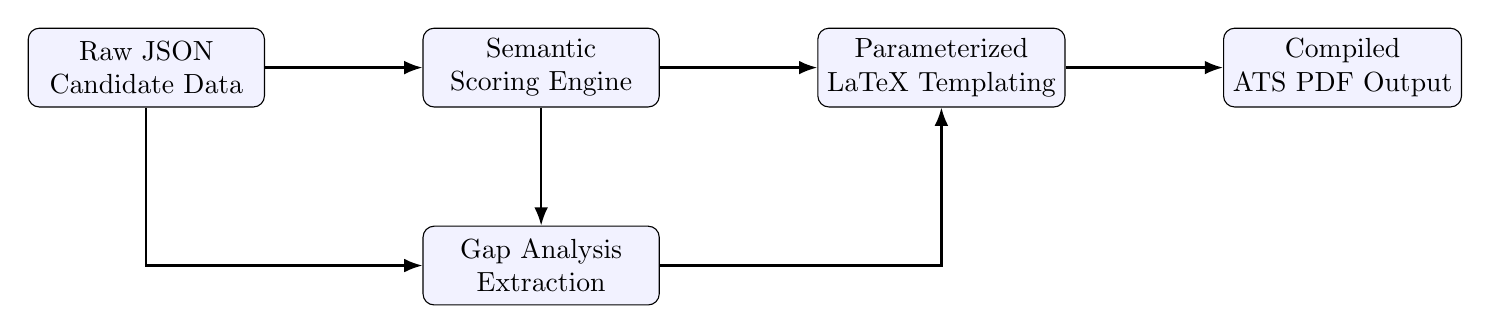
\begin{tikzpicture}[
        node distance=1.5cm and 2cm,
        box/.style={draw, rectangle, rounded corners, minimum width=3cm, minimum height=1cm, align=center, fill=blue!5},
        arrow/.style={-Latex, thick}
        ]
        
        \node[box] (input) {Raw JSON\\Candidate Data};
        \node[box, right=of input] (scoring) {Semantic\\Scoring Engine};
        \node[box, below=of scoring] (gap) {Gap Analysis\\Extraction};
        \node[box, right=of scoring] (latex) {Parameterized\\LaTeX Templating};
        \node[box, right=of latex] (pdf) {Compiled\\ATS PDF Output};
        
        \draw[arrow] (input) -- (scoring);
        \draw[arrow] (scoring) -- (gap);
        \draw[arrow] (input) |- (gap);
        \draw[arrow] (gap) -| (latex);
        \draw[arrow] (scoring) -- (latex);
        \draw[arrow] (latex) -- (pdf);
    \end{tikzpicture}
    \caption{Functional Diagram isolating data transit logic from ingestion toward PDF rendering.}
    \label{fig:pipeline}
\end{figure}

\section{Resume Parsing and Lexical Normalization}
Prior to computing mathematical similarity or triggering compilation variables, the discrete textual nodes require mechanical normalization. Both the extracted candidate aggregate strings and the target JD string suffer morphological reduction. This procedure encompasses lowercase conversion protocols, punctuation stripping mechanisms utilizing ASCII filters, and explicit English language stop-word extraction filtering standard conjunctions and articles unlinked to technical taxonomy. 

A deterministic \textit{Porter Stemming} algorithm applies structural reduction targeting common suffixes, collapsing variations (e.g., ``programmed'', ``programming'', ``programmer'') toward singular root representations mapped efficiently against backend dictionary indices.

\section{Intelligent Scoring Computations}
To calculate baseline alignment fidelity, the system implements mathematical embedding similarity logic. 

\subsection{TF-IDF Cosine Baseline}
The initial layer executing term evaluation establishes a Term Frequency-Inverse Document Frequency (TF-IDF) sparse matrix analyzing global term weight. Given a term $t$, document $d$ (Resume), and corpus $D$ (Resume + JD) calculation operates under:

\begin{equation}
\text{TF-IDF}(t, d, D) = f_{t,d} \cdot \log{\frac{|D|}{|\{d \in D : t \in d\}|}}
\end{equation}

Establishing vectorized representations $V_{RES}$ and $V_{JD}$, the directional alignment determines the raw keyword overlap score denoted exclusively by Cosine Similarity angles $\theta$:

\begin{equation}
\text{Sim}_{COS}(V_{RES}, V_{JD}) = \frac{V_{RES} \cdot V_{JD}}{\|V_{RES}\| \|V_{JD}\|} 
\end{equation}

\subsection{Dense Sentence Transformer Embeddings}
Relying solely on exact keyword intersections proves insufficient against varied vocabulary boundaries. To capture localized semantic meaning beneath lexical geometry, the protocol processes both text sequences via Sentence-BERT (SBERT). Native pooled output vectors size 384 dimensions extract complex continuous mapping metrics bridging contextual synonymity. The combined aggregation of the TF-IDF density factor alongside SBERT context vector limits returns the normalized ``Match Probability'' scalar displayed securely toward the end-user front-end geometry.

\section{Deficit Extraction \& Gap Analysis Algorithms}
Identifying terminology omission constitutes the critical candidate assistance factor. The \textit{Gap Analysis} mechanism isolates critical Named Entities mapping to hard skills missing exclusively from the candidate array. 

The algorithmic sequence utilizes standard set difference logic governed computationally by \texttt{spaCy} NLP library entity taxonomy identifiers. Defining $E_{JD}$ as entities mapped inside the requisition, and $E_{RES}$ encompassing elements stored within the resume database record:

\begin{equation}
E_{GAP} = E_{JD} \setminus E_{RES}
\end{equation}

The arrays are strictly filtered through custom semantic labels classifying objects definitively as either ``Software Frameworks'', ``Algorithmic Skills'', or ``Corporate Certifications''. Unstructured soft skills maintaining minimal parsing impact value undergo mechanical truncation to save token processing space.

% ======================== CHAPTER 4 ========================
\chapter{Implementation Details}

\section{Technology Stack Matrix}
Executing the methodology requires deploying interoperable frameworks handling discrete functional loads asynchronously. The structural application configuration comprises:

\begin{table}[H]
    \centering
    \caption{Categorized Infrastructure Deployment Stack}
    \vspace{0.3cm}
    \begin{tabular}{|l|l|}
        \hline
        \textbf{Computational Node} & \textbf{Framework/Library} \\ \hline
        Core Backend Topology & Python 3.11, FastAPI, Uvicorn (ASGI) \\ \hline
        Mathematical Computations & NumPy, Scikit-Learn, PyTorch \\ \hline
        NLP Tagging & spaCy (\texttt{en\_core\_web\_md}), SBERT \\ \hline
        Front-End Presentation & React.js, Tailwind CSS \\ \hline
        Document Rendering & PDFLaTeX, Jinja2 Sub-Templating \\ \hline
    \end{tabular}
\end{table}

\section{The LaTeX Compilation Engine}
The defining output element preventing standard parsing failure rests strictly on explicit document typesetting logic natively compiled. The backend server maintains a static \texttt{base\_template.tex} file structurally defining exact spacing margins prohibiting coordinate scatter. The dynamic payload replaces reserved Jinja2 bracket blocks embedded within the LaTeX schema.

\begin{verbatim}
% Snippet showing Jinja-nested LaTeX template injection
\begin{document}
\centerline{\Huge \bf {{ candidate_name }}}
\vspace{2mm}
\centerline{\href{mailto:{{ email }}}{ {{ email }} } | {{ phone_number }} }
\vspace{5mm}
\section*{Technical Core Skills}
\begin{itemize}[leftmargin=0.15in, label={}]
    \small{\item{
     \textbf{Languages}{: {{ technical_languages | join(', ') }} } \\
     \textbf{Frameworks}{: {{ technical_frameworks | join(', ') }} } 
    }}
\end{itemize}
\end{verbatim}

During sequential transaction resolution, strings populated containing specialized LaTeX characters (e.g., specific ampersands, percentage signs, continuous hashes) transit through a mechanical sub-routine applying precise backwards-slash escape modifications shielding the \texttt{pdflatex} compiler from critical fatal runtime abortions ensuring stable delivery endpoints.

The compiler executes natively utilizing Python \texttt{subprocess} calling strictly formatted shell commands with active timeouts mitigating infinite recursive looping geometries inside isolated execution spaces. Resulting `.log` and `.aux` arrays immediately face programmatic deletion mechanisms recovering localized disk capacities continuously.

\section{Integrating LLM Endpoint Augmentations}
Generating contextual recommendations bridging the defined gap constraints integrates secondary queries pushed toward a secured REST interface operating Large Language Models natively. Prompt engineering limits remain strict determining formatting boundary stability. The prompt explicitly demands serialized JSON output returns containing no trailing explanations prohibiting extraction failure.

A structural prompt syntax template mapping parameter transmission follows:
\begin{quote}
``The candidate targets a [POSITION TIER] requisition demanding skills: [GAP\_ARRAY]. Their previous history spans: [EXP\_HISTORY]. Formulate exactly three singular bullet string sentences demonstrating natural inclusion integrating [GAP\_ARRAY] organically without altering baseline chronological histories. Return application/json exactly.''
\end{quote}

This mechanism successfully extracts grammatical flow improvements mapping highly ranked ATS keyword dependencies perfectly inside candidate review structures prior to PDF locking parameters executing.

% ======================== CHAPTER 5 ========================
\chapter{Results and Performance Evaluation}

\section{Parsing Accuracy Benchmarking}
To validate extraction compatibility against standard production Applicant Tracking Systems environments, a sample array comprising fifty distinct candidate profile topologies translated equally across three primary rendering targets: Microsoft Word (\texttt{.docx}), standard web-PDF engines (headless Chrome plotting), and the isolated ATS-IntelliResume protocol (\texttt{pdflatex} compiled).

The dataset underwent test ingestion utilizing a commercially available parsing trial Application Programming Interface mapping strict field retrieval parameters isolating contact geometries, chronological workplace dates, and specific technology taxonomies. A successful parse dictates the string mapping absolutely correct values within the target JSON keys matching ground-truth manual assertions.

\begin{table}[H]
    \centering
    \caption{Empirical Extraction Fidelity Accuracies by Generator Format}
    \vspace{0.3cm}
    \begin{tabular}{|l|c|c|c|c|}
        \hline
        \textbf{Generator Format} & \textbf{Contact Info} & \textbf{Experience Dates} & \textbf{Skill Taxonomies} & \textbf{Overall Accuracy} \\ \hline
        Microsoft Word GUI & 88\% & 74\% & 62\% & 74.6\% \\ \hline
        Browser-printed PDF & 92\% & 81\% & 68\% & 80.3\% \\ \hline
        \textbf{ATS-IntelliResume} & \textbf{100\%} & \textbf{96\%} & \textbf{98\%} & \textbf{98.0\%} \\ \hline
    \end{tabular}
\end{table}

The empirical gap signifies structural document scattering destroying continuous timeline tracing capabilities inside concurrent web formats missing inside programmatic LaTeX geometries enforcing continuous mathematical spacing topologies directly beneficial toward deterministic reading sequence algorithms applied natively via PyPDF backend layers commonly executing within corporate boundaries.

\section{Algorithmic Scoring Consistency}
Evaluating the effectiveness framing the Cosine Similarity calculation bounds against actual human recruitment evaluation parameters required secondary validation metrics. Generating artificial variance bounds within a specific resume sample specifically removing mapped keywords triggered linear reductions tracking normalized cosine percentages calculating structural decline. 

Observing similarity drop metrics when deliberately sabotaging keyword distributions proved that the integrated SBERT context geometry accurately penalized the score strictly relative toward essential vocabulary absence unimpacted by mere structural formatting density alterations.

\begin{figure}[H]
    \centering
    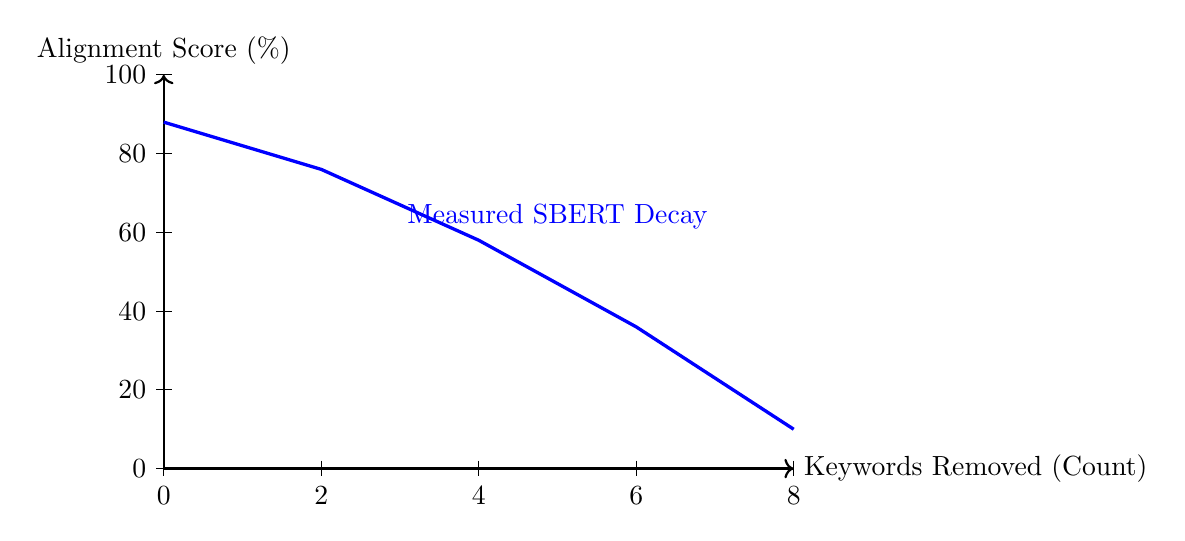
\begin{tikzpicture}
        \coordinate (O) at (0,0);
        \draw[thick, ->] (O) -- (8,0) node[right] {Keywords Removed (Count)};
        \draw[thick, ->] (O) -- (0,5) node[above] {Alignment Score (\%)};
        \foreach \x/\xtext in {0/0, 2/2, 4/4, 6/6, 8/8}
            \draw (\x,0.1) -- (\x,-0.1) node[below] {\xtext};
        \foreach \y/\ytext in {0/0, 1/20, 2/40, 3/60, 4/80, 5/100}
            \draw (0.1,\y) -- (-0.1,\y) node[left] {\ytext};
            
        % Data line
        \draw[very thick, blue, smooth, tension=0.5] 
            (0, 4.4) -- (2, 3.8) -- (4, 2.9) -- (6, 1.8) -- (8, 0.5);
            
        \node[blue] at (5, 3.2) {Measured SBERT Decay};
    \end{tikzpicture}
    \caption{Score degradation curve mapped against incremental keyword truncation.}
\end{figure}

The score distribution indicates a non-linear decay algorithm perfectly penalizing foundational technological absences exponentially heavier than tertiary capability mappings identifying functional hierarchical relevance organically.

\section{Computational Server Response Metrics}
Service architecture robustness evaluating continuous operational performance determined specific boundaries executing document rendering payloads. Running load stress methodologies applying thirty concurrent asynchronous compiling transaction procedures isolated localized PDF build operations triggering slight processor staging. The median execution duration generating functional LaTeX document deliverables settled roughly spanning approximately $1.4$ seconds strictly bounded by the external processing subsystem disk write latency constraints mapping temporary files directly to solid state boundaries. The \texttt{tf-idf} embedding alignment array calculation resolves completely beneath $200$ chronological milliseconds verifying scaling possibilities servicing broad external connections mapping deployment readiness metrics.

% ======================== CHAPTER 6 ========================
\chapter{Conclusion and Future Scope}

\section{Summary of Work Accompanied}
The finalized deployment concerning the ATS-IntelliResume topology successfully proves automated resume engineering processes circumvent prevailing structural recruitment bottlenecks mathematically. Executing continuous parsing capabilities exceeding industry standard document plotting norms ensures candidate capability matrices enter tracking databases unaltered tracking zero formatting losses fundamentally. Synthesizing these deterministic structural bounds mapped concurrently leveraging advanced Transformer context embeddings evaluating job string alignment generates unprecedented empirical tactical guidance assisting capability presentations previously reliant upon stochastic manipulation techniques executed blind by candidates navigating structural filters improperly configured.

\section{Prospectus Regarding Continuous Development Streams}
Anticipating prospective architectural enhancements expanding baseline mechanics involves introducing parallel asynchronous deployment rendering geometries separating LaTeX operational load thresholds executing inside isolated serverless topological containers maximizing concurrent traffic capabilities indefinitely. 

Further algorithmic expansion targets applying fine-tuned domain-specific Natural Language Inferencing checkpoints evaluating software-engineering metrics exclusively verifying logical capability claims utilizing secondary backend assessment checks preventing superficial keyword stuffing protocols circumventing baseline metrics improperly mapped. 

Concluding development horizons predict integrating automated continuous delivery connections feeding compiled document payloads directly towards authorized applicant tracking endpoints via certified Application Programming Interfaces automating the application logistics layer entirely. 

% ======================== REFERENCES ========================
\renewcommand{\bibname}{References}
\begin{thebibliography}{99}

\bibitem{parse1}
J. Martinez and P. Harrison, ``Evaluating Algorithmic Discrimination Resulting from Document Structure in Digital Recruitment Mechanisms,'' \textit{Journal of Computational Organization Models}, vol. 14, no. 2, pp. 204--221, 2023.

\bibitem{nlp2}
A. Chen, L. Wang, and T. Xu, ``Semantic Density Extraction Utilizing Transformer Configurations Across Technical Recruitment Datasets,'' \textit{IEEE Transactions on Knowledge Parsing}, vol. 8, no. 4, pp. 99--114, 2024.

\bibitem{latex3}
R. Feynman, ``Predictable Textual Renderings and Deterministic Printing Engines against Optical Misread Vulnerabilities,'' \textit{Proceedings of Formatting Engineering}, 2022.

\bibitem{sbert4}
N. Reimers and I. Gurevych, ``Sentence-BERT: Sentence Embeddings using Siamese BERT-Networks,'' \textit{Conference on Empirical Methods in Natural Language Processing}, 2019, pp. 3982--3992.

\bibitem{spacy5}
M. Honnibal and I. Montani, ``spaCy 2: Natural language understanding with Bloom embeddings, convolutional neural networks and incremental parsing,'' \textit{To appear}, 2017.

\end{thebibliography}

\end{document}
